\section{Fluxional execution model} \label{section:model}

The tool we present in this paper transforms a monolithic application into a network of autonomous parts communicating by message streams.
There exist many execution models designed for such distributed system renowned precisely for their performances\cite{Welsh2000, Jain2006, Wu2007, Zaharia2010, Akidau2013, Marz2011}.
However, we focus on a compilation approach to replace the shift in programming model rather than the performance of the runtime.
Therefore, we present in this section an extremely simplified execution model inspired by the literature, only to support the confirmation of feasibility for the compilation process detailed in section \ref{section:compiler}.

\subsection{Fluxions}

The fluxional execution model role is to manage and invoke autonomous execution units.
An execution unit listens for, and sends back streams.
A stream is a continuous and infinite sequence of data encapsulated in messages.
We named this execution unit a fluxion, by contraction between a flux and a function.
A fluxion is a function, as in functional programming, consuming an input stream and generating one or more outputs streams.
It is composed of a unique name, a processing function, and a persisted memory \textit{context}.

Messages are carried between fluxions by a messaging system.
They are composed of the name of the recipient fluxion and a body.
At a message reception, the fluxion modifies its memory \textit{context}, and sends back messages to downstream fluxions.
The memory \textit{context} of a fluxion contains all of the state variables on which the fluxion depends between two executions - that is two message receptions.

The fluxions form a processing chain linked by message streams.
All these chains constitute a directed graph, operated by the messaging system.

\subsection{Messaging system}

The messaging system is the core of our fluxional execution model.
It carries messages along streams, and invokes fluxions at a message reception.

The messaging system is built around a message queue.
Each message is processed one after the other by invocation of the destination fluxion.
% Using a message queue allows to execute multiple processing chains fairly and concurrently, without difference in scheduling local messages, or network messages.
The life cycle of a fluxional application is pictured on figure \ref{fig:MesSys}.

\begin{figure}[h!]
  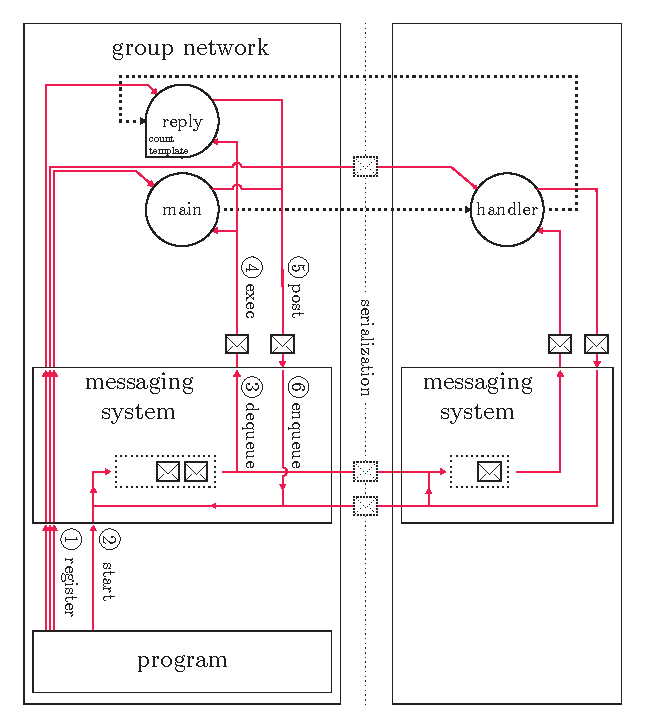
\includegraphics[width=\linewidth]{ressources/schema-message.pdf}
  \caption{Messaging system details}
  \label{fig:MesSys}
\end{figure}

The messaging system carries message streams based on the names of the recipient fluxions.
So it needs every fluxion to be registered.
If two fluxions share a name, the messaging system would be in a conflicting situation.
This registration associates a processing function with a unique name and an initial memory \textit{context}.
The registration is done using the function \texttt{register(<nom>, <fn>, <context>)}, step \circled{1}.
% A fluxion can dynamically register other fluxions

To trigger a chain of fluxions, a message is sent using the function \texttt{start(<msg>)}, step \circled{2}.
This function pushes a first message in the queue.
Immediately, the system dequeues this message to invoke the recipient processing function, step \circled{3} and \circled{4}.
The recipient function sends back messages using the function \texttt{post(<msg>)}, step \circled{5}, to be enqueued in the system, step \circled{6}.
The system loops through steps \circled{3} and \circled{4} until the queue is empty.
This cycle starts again for each new \textit{start} message.

The algorithms \ref{alg:parcours} and \ref{alg:traitement} describe the behavior of the messaging system after the function \texttt{start} invocation.

\begin{algorithm}
\caption{Message queue walking algorithm}
\label{alg:parcours}
\begin{algorithmic}
\Function{loopMessage}{\null}
\While{$msg$ \textbf{presents in} $msgQueue$}
\State $msg \gets$ \Call{dequeue}{\null} \Comment{\circled{3}}
\State \Call{ProcessMsg}{$msg$}
\EndWhile
\EndFunction
\end{algorithmic}
\end{algorithm}

\begin{algorithm}
\caption{Message processing algorithm}
\label{alg:traitement}
\begin{algorithmic}
\Function{processMsg}{$msg$}
\For{$dest$ \textbf{in} $msg.dest$}
\State $fluxion \gets lookup(dest)$
\State $message \gets$ \Call{exec}{$fluxion, msg.body$} \Comment{\circled{4} \& \circled{5}}
\State \Call{enqueue}{$message$} \Comment{\circled{6}}
\EndFor
\EndFunction
\end{algorithmic}
\end{algorithm}

\subsection{Service example}

To illustrate the fluxional execution model, we present an example of a simple web application.
This application sends back its own source along with a request counter.

\includecode{js,
  caption={Simple web application. \textnormal{this application replies to every user request with its own source code and the value of a request counter}},
  label={lst:ex-source}
}
{../../example/source.js}

The original source code of this application is available on github\cite{flx-example}\footnote{\raggedright https://github.com/etnbrd/flx-example/releases}, and in listing \ref{lst:ex-source}.
In this source code, some points are worth noticing.

\begin{itemize}
  \item The \texttt{reply} function, line 5 to 11, contains the logic we want to split into the fluxional processing chain.
  It receives the user request in the variable \texttt{res} which is used by the last element of the chain.
  \item The \texttt{count} object at line 3 is a persistent memory that increment the request counter.
  This object needs to be mapped to a fluxion \textit{execution context} in the fluxional execution model.
  \item The two functions \texttt{get} and \texttt{send}, respectively line 5 and 9, interfaces the application with the clients.
  The processing chain of functions is in between these two functions : $\texttt{get} \to \texttt{handler} \to \texttt{readFile} \to \texttt{reply} \to \texttt{send}$.
\end{itemize}

This application is transformed manually into the fluxions chain depicted in Figure \ref{fig:fluxions}.
We expect a similar result with the compiler described in section \ref{compiler}.
The circles represent registered fluxions.
Envelope symbols represent messages streams between fluxions with the variables transmitted from one fluxion to the other.
The square in the messaging system holds the memory \textit{context} of the \texttt{reply} fluxion.
When a new \texttt{GET} REST request is received by the starting fluxion named \texttt{get}, a \texttt{start} message triggers the flow.
The \texttt{handler} fluxion receives this \texttt{start} message, read the source file and forward it to the \texttt{reply} fluxion which increments the counter, and sends the result back.
Each fluxion propagates the necessary values from one fluxion to the other exclusively by messages.
Horizontal dashed lines show virtual transmission of messages between fluxions although they all go through the messaging system.

\begin{figure}[h!]
  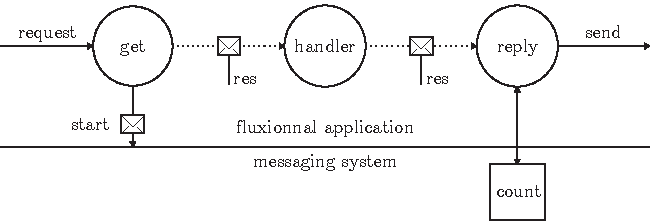
\includegraphics[width=\linewidth]{ressources/flux.pdf}
  \caption{Fluxions chain manually extracted from the example application}
  \label{fig:fluxions}
\end{figure}

Listing \ref{lst:fluxional} describes this counting application in our high-level fluxional language.
This language brings a stricter segmentation than the initial code by allowing to only register and define fluxions.
In this language, a fluxion is defined by a name, a description of the memory \textit{context}, the operator \texttt{>}\texttt{>} for starting fluxions or \texttt{-}\texttt{>} for following fluxions and finally a list of downstream fluxions with the content of the message for each stream.
The body containing the processing function is following the fluxion definition.
It uses the Javascript language syntax, and is indented with 2 spaces to improve readability.
The processing function can access and manipulate only two objects : \texttt{msg} and \texttt{this}.
The first is the received message, the second is the persisted \textit{context} of the fluxion.
There is an exception for the starting fluxion whose body isn't a function, because it never receives any stream, but is only executed once to initialize the application.

\begin{code}[flx, caption={Manual transformation of the example application in our high-level fluxional language},label={lst:fluxional}]
flx get
>> handler [res]
  var app = require('express')(),
      fs = require('fs'),
      count = 0;

  app.get('/', >> handler);
  app.listen(8080);
  console.log('>> listening 8080');

flx handler
-> reply [res]
  function handler(req, res) {
    fs.readFile(__filename, -> reply);
  }

flx reply {count}
-> null
  function reply(error, data) {
    count += 1;
    var code = ('' + data).replace(/\n/g, '<br>').replace(/ /g, '&nbsp');
    res.send('downloaded ' + count + ' times<br><br><code>' + code + '</code>');
  }
\end{code}

The application is organized as follow :
\begin{itemize}
  \item The \texttt{get} fluxion is the starting fluxion.
  It initializes the application to listen for user request calling \texttt{app.get}.
  Every request is sent to the \texttt{handler} request.
  \item The \texttt{handler} fluxion reads the source file to send it to the user, and forwards the result to the \texttt{reply} fluxion.
  \item The \texttt{reply} fluxion increments the counter, formats the reply, and sends it back to the user using the function \texttt{res.send}.
\end{itemize}

Our goal, as described in the introduction, is not to propose a new programming paradigm with this high-level language but to automate the architecture shift with a compiler.